\section{同洗牌条件消耗收益的分布}\label{sec:conditional}
\subsection{由设置阶段计数构造联合概率}
两阶段样本来自同一排列。第一阶段抽走的类别数量，决定第二阶段的剩余组成，
所以应先给定设置阶段计数，再对条件分布求混合。
在基准中，成功时A、B均已揭示。
设前10张的C、S数量分别为$c_1,s_1$，其余为D或T，共有10张可选。
这些计数与$I=1$同时发生的无条件概率为
\begin{equation}\label{eq:setup-counts}
q(c_1,s_1)=
\frac{\binom2{c_1}\binom{10}{s_1}\binom{10}{8-c_1-s_1}}{\binom{24}{10}},
\qquad c_1\in\{1,2\},\quad 0\le s_1\le10.
\end{equation}
计数式中的组合数自动排除越界情况，$q$在全部设置计数上的和为$p$。
剩余$L=N-n=14$张中，可被C消耗的牌数为
$M(c_1,s_1)=(2-c_1)+(10-s_1)=12-c_1-s_1$。
给定计数后，未揭示部分仍是均匀排列，故
\begin{equation}\label{eq:hypergeometric}
\Prob(X=x\mid c_1,s_1,I=1)=
\frac{\binom{M(c_1,s_1)}x\binom{14-M(c_1,s_1)}{4-x}}{\binom{14}4},
\qquad x=0,\ldots,4.
\end{equation}
对互斥的设置阶段计数求和，得到联合概率质量
\begin{equation}\label{eq:joint}
J_x:=\Prob(X=x,I=1)=
\sum_{c_1=1}^2\sum_{s_1=0}^{10}q(c_1,s_1)
\frac{\binom{12-c_1-s_1}x\binom{2+c_1+s_1}{4-x}}{\binom{14}4}.
\end{equation}
每个超几何分布均归一，因此
$\sum_xJ_x=\sum_{c_1,s_1}q(c_1,s_1)=p$；
成功条件下的PMF为$J_x/p$，其权重为$q(c_1,s_1)/p$。

也可以先枚举收益位置$n+1,\ldots,n+h$的类别计数，
再从剩余实体中计算设置阶段的可及性。
两种条件化次序都得到$J_x$；研究中以精确有理数和小牌组全排列完成交叉验证。

\subsection{条件矩、尾概率与总体零收益}
基准条件PMF依次为
\begin{equation}\label{eq:conditional-pmf}
\bigl(\Prob(X=x\mid I=1)\bigr)_{x=0}^4
=\left(\frac{54}{1615},\frac{128}{595},\frac{933}{2261},
        \frac{636}{2261},\frac{130}{2261}\right).
\end{equation}
对式\eqref{eq:conditional-pmf}按$x$及$x^2$加权，
再将消耗数均值乘8、方差乘64，可得
\begin{equation}\label{eq:conditional-moments}
\begin{aligned}
\E(X\mid I=1)&=\frac{74}{35},\qquad
\V(X\mid I=1)=\frac{19716}{23275},\\
\mu&=\frac{592}{35}\approx\BaseMu,\qquad
\sigma^2=\frac{1261824}{23275}\approx\BaseConditionalVar.
\end{aligned}
\end{equation}
条件标准差约为7.3630，且
$\Prob(G\ge24\mid I=1)=766/2261\approx\BaseTail$。
对应的总体阈值概率为
$\Prob(Y\ge24)=p\Prob(G\ge24\mid I=1)\approx\BaseOverallTail$。
该式直接由联合事件$\{Y\ge24\}=\{I=1,G\ge24\}$得到。

\begin{figure}[htbp]
\centering
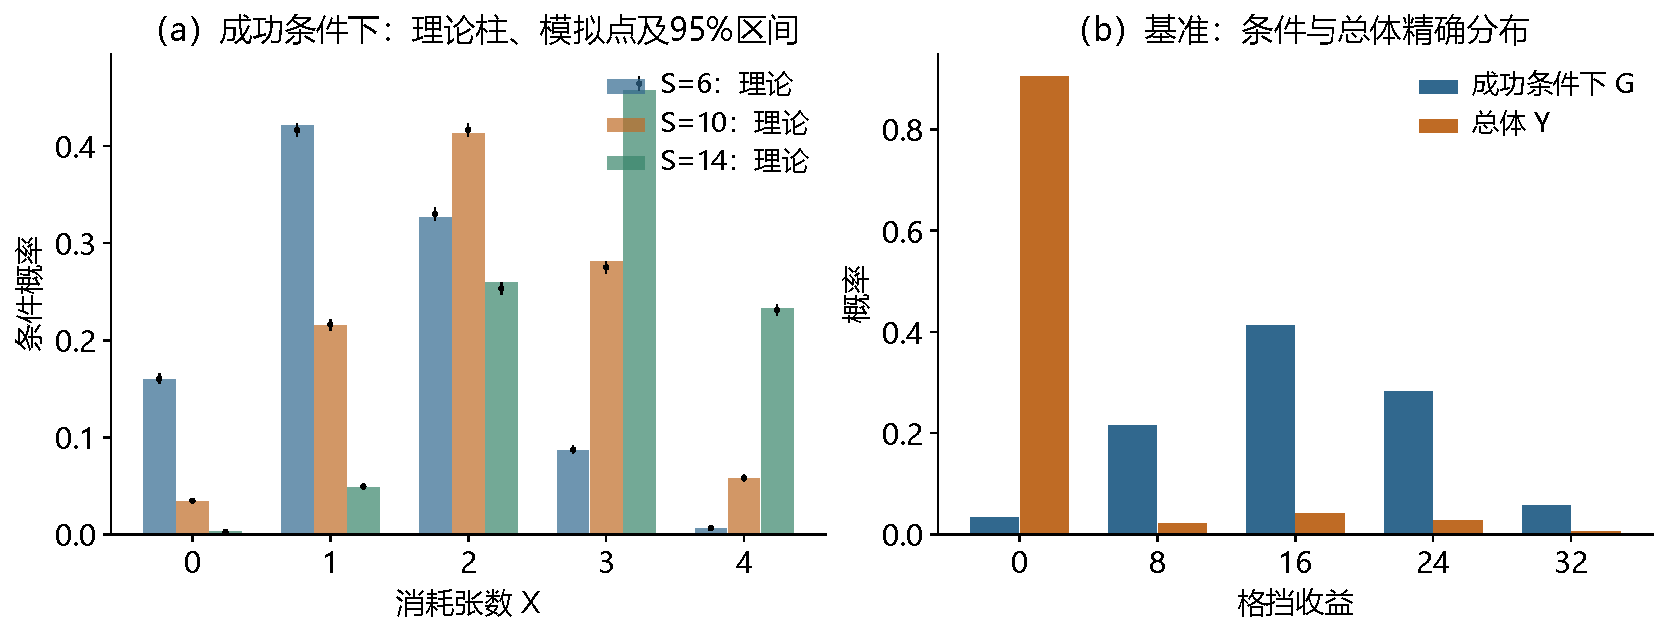
\includegraphics[width=\linewidth]{04_payoff_distributions.pdf}
\caption{条件消耗数量与收益分布。左图柱为精确理论值，点与区间来自每配置20万次模拟；
右图比较基准条件收益与总体收益的精确PMF。}\label{fig:distribution}
\end{figure}

图\ref{fig:distribution}右图的总体零收益概率为
\begin{equation}\label{eq:zero}
\Prob(Y=0)=1-p+J_0=\frac{73914}{81719}\approx\BaseZero.
\end{equation}
它同时包含组件未齐与组件齐全后$X=0$两种情况。
因此，基准总体90\%分位数为0，而条件90\%分位数为24。
更一般地，若$p\le0.1$，则$\Prob(Y=0)\ge1-p\ge0.9$，
非负总体收益的90\%分位数必为0。
对于这种零值集中的分布，阈值概率和条件分位数能补充总体分位数的区分能力。

\subsection{条件混合与独立重抽的区别}
若预先确定并移除一张A、B、C，再从剩余21张中重新均匀抽4张，
可消耗牌数为11，所定义的另一实验服从
$\operatorname{Hypergeom}(21,11,4)$，格挡均值为$352/21\approx16.761905$。
它与式\eqref{eq:conditional-moments}的差别，来自对前10张随机计数的不同处理。
独立重抽模型若沿用原协议的$p$，总体均值为1.656315；
同洗牌模型则为1.671372。两种抽样方式产生不同的条件分布。

条件混合的方差也有可解释的两层结构。
令$W=(c_1,s_1)$，$\theta=M(W)/L$。
在$L>1$时，超几何方差与全方差公式给出
\begin{equation}\label{eq:mixture-variance}
\V(X\mid I=1)=
h\frac{L-h}{L-1}\E\!\left[\theta(1-\theta)\mid I=1\right]
+h^2\V(\theta\mid I=1).
\end{equation}
式\eqref{eq:joint}的混合分布同时反映两层波动：
给定剩余组成后的无放回抽样波动，以及剩余组成本身的随机性。
